\section{Simulation Analysis}
\label{sec:simulation}

In this section, Ngspice was used in order to simulate the audio converter, therefore, a brief description of the circuit modeled in NGspice is going to be presented and a comparison between the values obtained in NGspice and the ones in Octave is going to be done as well. In order to do that, transistors of the given models were used and the rest of the components specifications changed to be on par with the values through MatLab.

In the next sections we are interested in the two impedances associated with the circuit as a whole ($Z_in$ and $Z_out$), both cut-off frequencies ($f_{CO_L}$ and $f_{CO_H}$), the bandwidth (interval between the cut-off frequencies) and the total gain ($A_V$) measured in the bandpass region. The measurement of these parameters and the overall performance of the circuit is outlined in 3.
We also confirm whether the BJTs are on the Forward Active Region (FAR), by comparing $V_CE$ and $V_BE$ for the NPN (and, analogously, $V_EC$ and $V_EB$ for PNP).
The confirmation is presented below:


\subsection{Coupling Capacitor}

In our Amplifier circuit there are two coupling capacitors ($C_in$ and $C_O$) but, since their functions are equivalent, we will focus on the first capacitor, the $C_in$ . Below, is shown 2 figures of the frequency response analysis, just by changing the parameter C drastically.

%\begin{figure}[H] 
%\centering
%\begin{subfigure}{0.4\textwidth}
%\includegraphics[width=\textwidth]{}
%\caption{High $C_in$}
%\label{highcin}
%\end{subfigure}
%\begin{subfigure}{0.3\textwidth}
%\includegraphics[width=\textwidth]{}
%\caption{Low $C_in$}
%\label{lowcin}
%\end{subfigure}
%\caption{$C_in$ influence}
%\end{figure}

As expected, the increase of the capacitance pushes the cutoff frequency to the left,
without changing the higher cut-off frequency, which leads to a larger bandwidth. \par
As discussed previously, as $\omega$ tends to 0, the impedance Z($C_in$) will tend to infinite, so this
capacitor prevents the transistor from entering on either the saturation or cut-off regions, by blocking the DC component of the AUDIO IN source. This helps mantaining the Operating Point of the transistor, so that it can operate at lower frequencies, as the value of $C_in$ increases.

\subsection{Bypass Capacitor}

In our Amplifier circuit there is one bypass capacitor ($C_E$).\par 
Below, is shown 2 figures of the frequency response analysis, just by changing the parameter $C_E$.

%\begin{figure}[H] 
%\centering
%\begin{subfigure}{0.4\textwidth}
%\includegraphics[width=\textwidth]{}
%\caption{High $C_E$}
%\label{highce}
%\end{subfigure}
%\begin{subfigure}{0.3\textwidth}
%\includegraphics[width=\textwidth]{}
%\caption{Low $C_E$}
%\label{lowce}
%\end{subfigure}
%\caption{$C_E$ influence}
%\end{figure}

As expected, by placing the bypass capacitor in parallel with $R_E$ , this resistor becomes a short circuit for medium and high frequencies (because the capacitor impedance is 1/(j$\omega$C) and $\omega$ = 2$\pi$f). The amplifier’s first stage gain is inversely dependent on this resistance, being that the bypass capacitor plays a very important role in maximizing the gain for medium and high frequencies.

\subsection{$R_c$}

In this subsection we will analyse the importance of $R_C$ on the total Gain of the circuit.
We also present assymptotical situations in order to fully understand that behaviour, 

%\begin{figure}[H] 
%\centering
%\begin{subfigure}{0.4\textwidth}
%\includegraphics[width=\textwidth]{}
%\caption{High $R_C$}
%\label{highrc}
%\end{subfigure}
%\begin{subfigure}{0.3\textwidth}
%\includegraphics[width=\textwidth]{}
%\caption{Low $R_C$}
%\label{lowrc}
%\end{subfigure}
%\caption{$R_C$ influence}
%\end{figure}

Analysing the figures, we can conclude that the gain increases with $R_C$ and also antecipates the passband.
This behaviour was already expected, because as described previous in the theorectical analysis of the gain, $R_C$ is proportional to the gain.
It is also important, in order to guarantee a high compatibility with AUDIO IN and to the 
speakers itself, to simulate the input and output impedances of the circuit. A good compatibility is ensured with a very high input impedance ($Z_in$) and a very low output impedance ($Z_out$). \par 
The following tables show the simulation results obtained of $Z_in$ and $Z_out$ respectively.

%\begin{table}[H] \centering
%\begin{tabular}{|
%>{\columncolor[HTML]{FFCC67}}l |c|}
%\hline
%\multicolumn{2}{|l|}{\cellcolor[HTML]{EABD8B}Name - Value} \\ \hline
%Zin & 999.002 + -7.3282 j\\ \hline

%\end{tabular}
%\caption{Results for the output of the envelope}
%\end{table}

%\begin{table}[H] \centering
%\begin{tabular}{|
%>{\columncolor[HTML]{FFCC67}}l |c|}
%\hline
%\multicolumn{2}{|l|}{\cellcolor[HTML]{EABD8B}Name - Value} \\ \hline
%\input{../sim/Zout_tab}
%\end{tabular}
%\caption{Results for the output of the envelope}
%\end{table}

As said theoretically, the load's impedance is equal to 8$\Omega$ . The value of $Z_out$ should be lower than this value. Given that the output value of the simulation is higher, this is going to compromise the value of the merit.

\subsection{Comparison}

Now that we have established the concepts theoretically and shown the simulation results, we are going to do a comparison between the two approaches (theoretically and simulation) with the chosen values for the constants. \par
The next graphs show the theoretical and simulation graphs of the gain respectively:

%\begin{figure}[H] 
%\centering
%\begin{subfigure}{0.4\textwidth}
%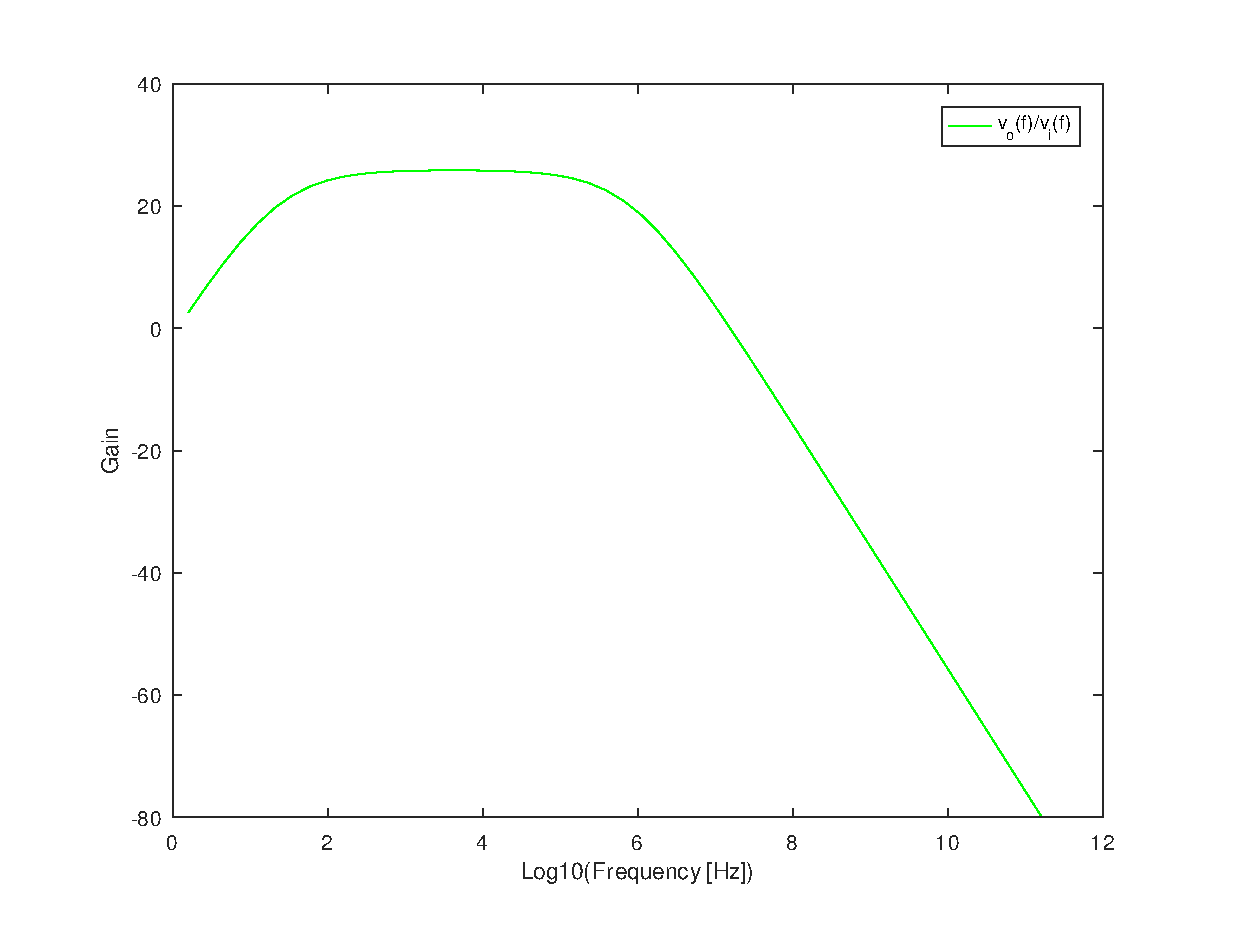
\includegraphics[width=\textwidth]{Gain.eps}
%\caption{Octave}
%\label{fig:first}
%\end{subfigure}
%\begin{subfigure}{0.3\textwidth}
%\includegraphics[width=\textwidth]{}
%\caption{NgSpice}
%\label{fig:second}
%\end{subfigure}
%\caption{Output AC Component}
%\end{figure}

In this case, the comparison of the shape can only be done on the left side, since we don’t
have the theoretical higher cut-off frequency. For this reason, there’s no point in plotting the
theoretical gain any further than 1M Hz.
One should bear in mind that the theorectical analysis either considers the capacitors are
short-circuited or are open-circuited (this approximation is made when for this analysis, the
value of R E is either 0 or R E in Table 1, respectively). For this reason, two estimates were
made (Figure 7) - in blue the capacitors are considered short-circuited; in orange the capacitors
are considered open-circuited; in yellow dashed it is represented the medium-value plot, that
can be considered as a rough approximation of the real gain. This theorectical approach does
not guarantee a specific value for the overall gain, however it gives us a region of acceptable
gains. The simulation gain obtained is satisfyingly in this prediction region.
The overall shape of the graphs is similar, noting that the theoretical one can be thought of
as assymptotical rather than a precise approach. In fact, as we imposed its shape, accordingly
to the one given by Ngspice, it is not sensible to variations that might occur (as the appearance
of a second step in 6b).
In a greater detail analysis, when remembering the values presented in the previous sub-
sections - Z I and Z O , A v and f CO L -, despite the obvious differences, the comparison is sat-
isfactory. Comparing the order of magnitude, when putting values side by side, they are within
reasonable intervals of similarity. In fact, the lower cut-off frequencies (from tables 5 and 8) are
really close, especially when you remember they are to be plotted in a logscale graph.
In conclusion, the theoretical approach gives a rough perspective of the overall work condi-
tions of the amplifier, which is good in a first sketch.


%\begin{table}[H] \centering
%\begin{tabular}{|
%>{\columncolor[HTML]{FFCC67}}l |c|}
%\hline
%\multicolumn{2}{|l|}{\cellcolor[HTML]{EABD8B}Name - Value} \\ \hline
%V_CE&4.71217\\ \hline
V_BE&0.642988\\ \hline
V_CE>V_BE & Correct F.A.R\\ \hline

%\end{tabular}
%\caption{NPN}
%\end{table}

%\begin{table}[H] \centering
%\begin{tabular}{|
%>{\columncolor[HTML]{FFCC67}}l |c|}
%\hline
%\multicolumn{2}{|l|}{\cellcolor[HTML]{EABD8B}Name - Value} \\ \hline
%V_CE&6.83806\\ \hline
V_EB&0.785099\\ \hline
V_EC>V_EB & Correct F.A.R\\ \hline

%\end{tabular}
%\caption{PNP}
%\end{table}

%\begin{table}[H] \centering
%\begin{tabular}{|
%>{\columncolor[HTML]{FFCC67}}l |c|}
%\hline
%\multicolumn{2}{|l|}{\cellcolor[HTML]{EABD8B}Name - Value} \\ \hline
%V-Gain & 34.1988\\ \hline
Bandwidth & 1.22501E+06\\ \hline
CO-lowerFreq & 15.8734\\ \hline
CO-higherFreq & 1.22503E+06\\ \hline

%\end{tabular}
%\caption{Results for the output}
%\end{table}

\begin{figure}[H] 
\centering
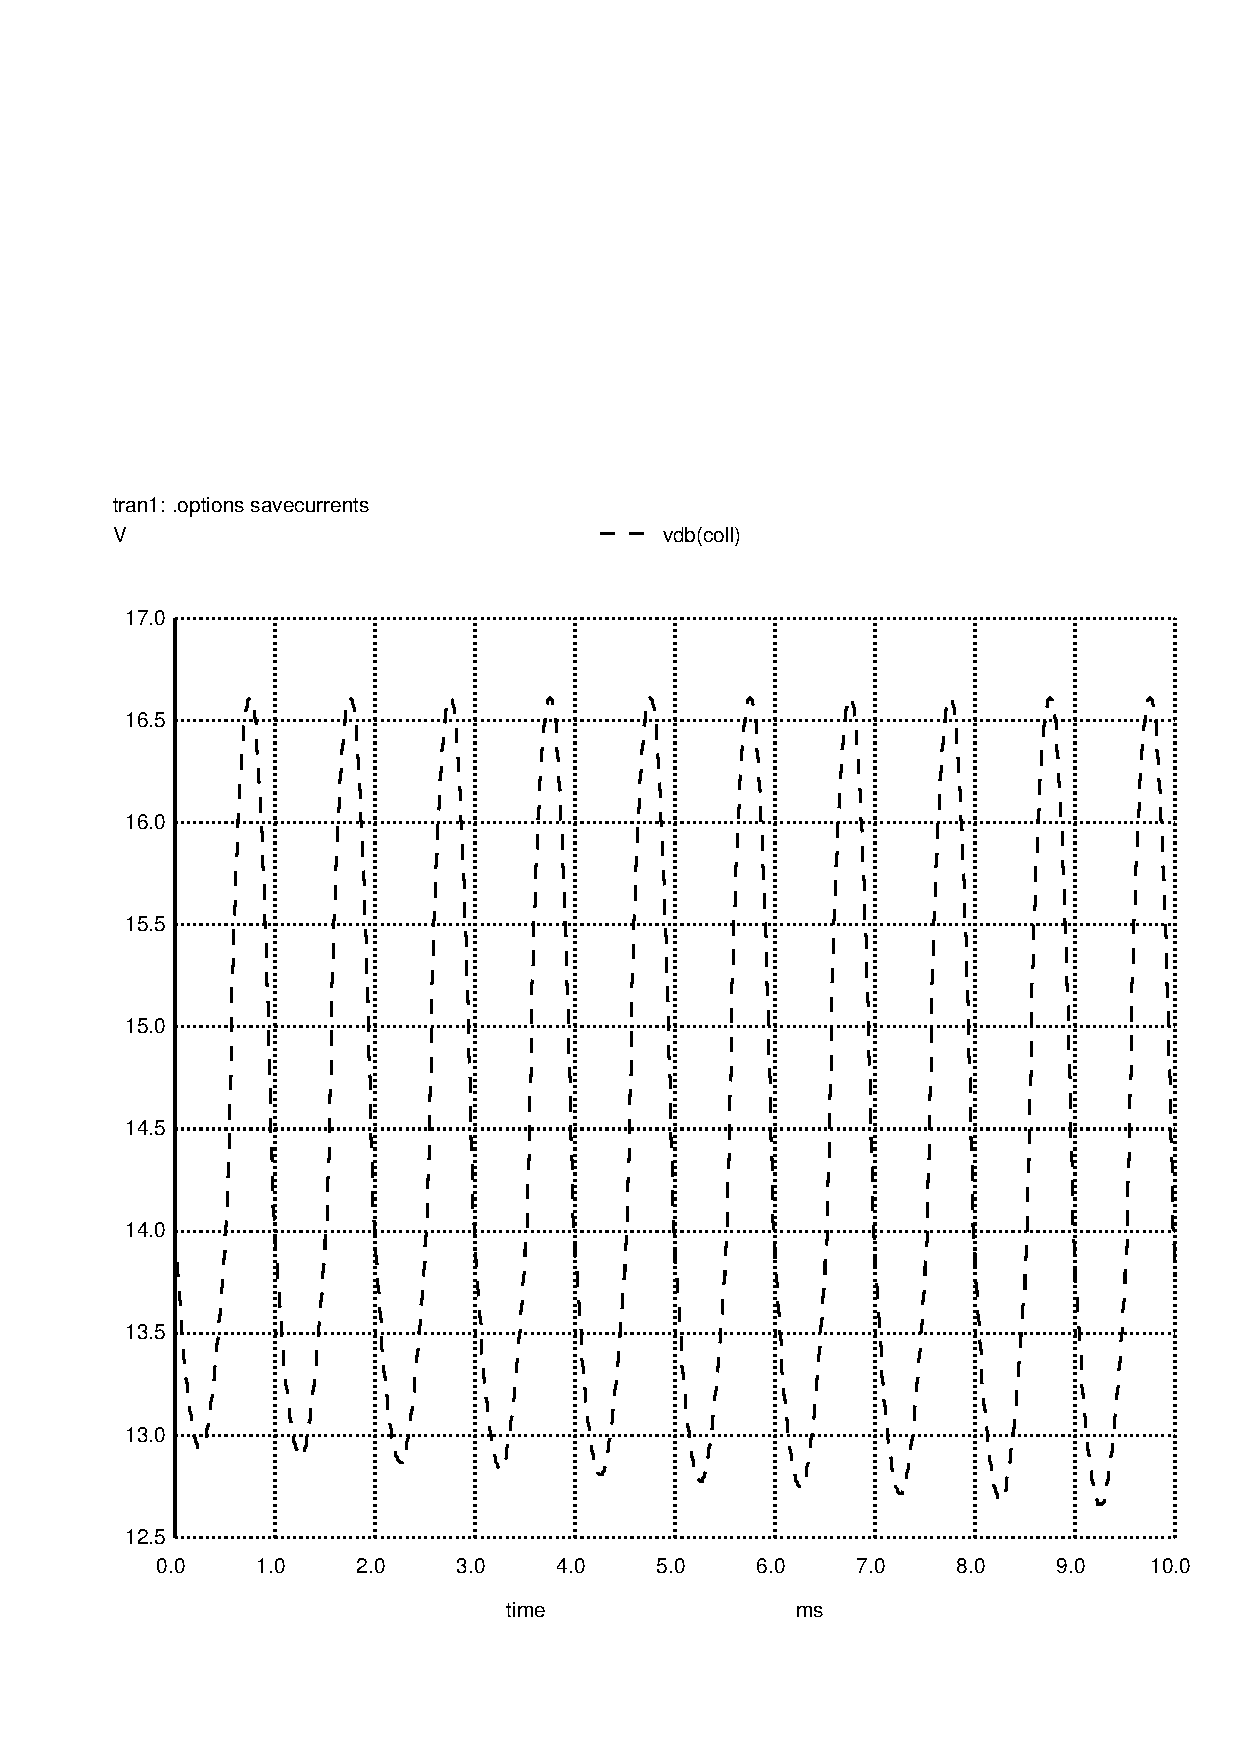
\includegraphics[width = 8cm]{vo1.pdf} 
\caption{Output}
\label{vo1}
\end{figure}

\begin{figure}[H] 
\centering
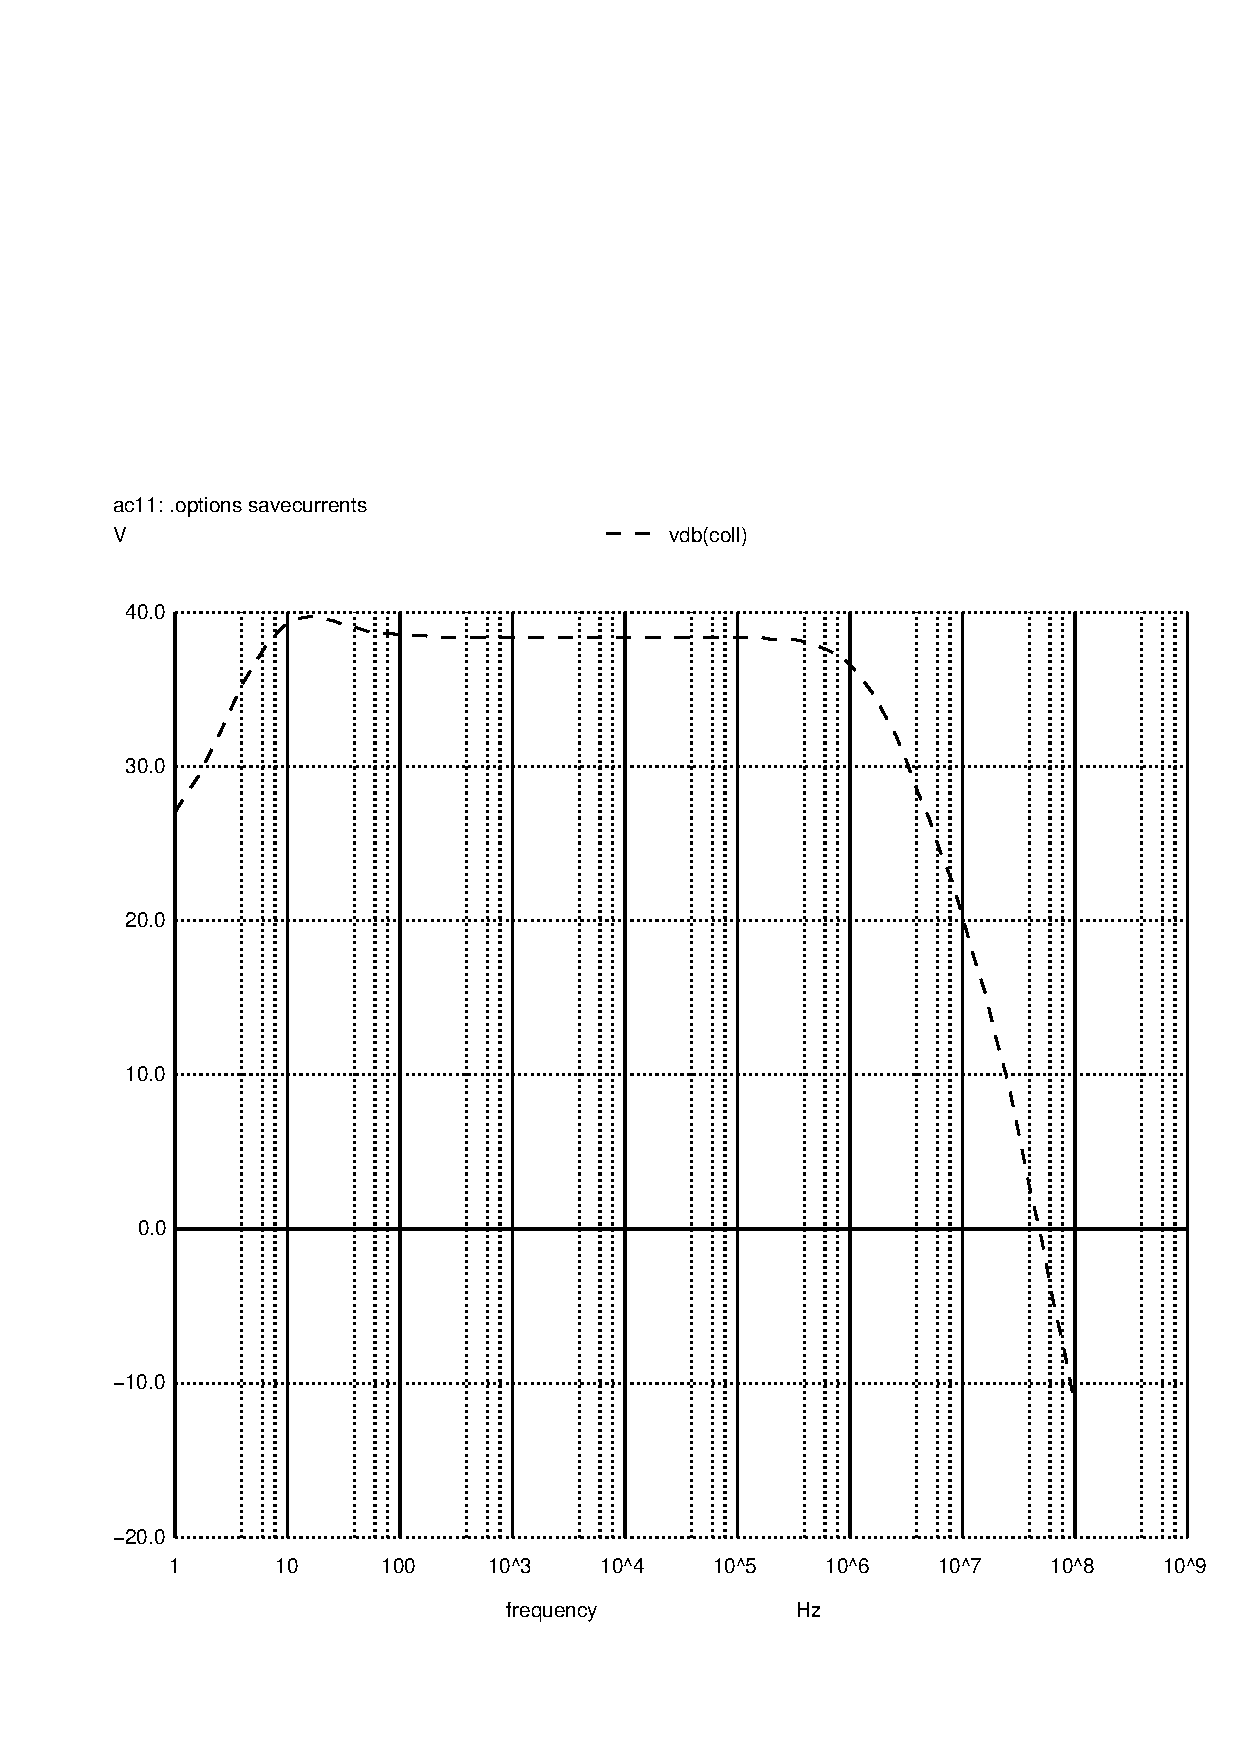
\includegraphics[width = 8cm]{vo1f.pdf} 
\caption{Output}
\label{vo1f}
\end{figure}

\begin{figure}[H] 
\centering
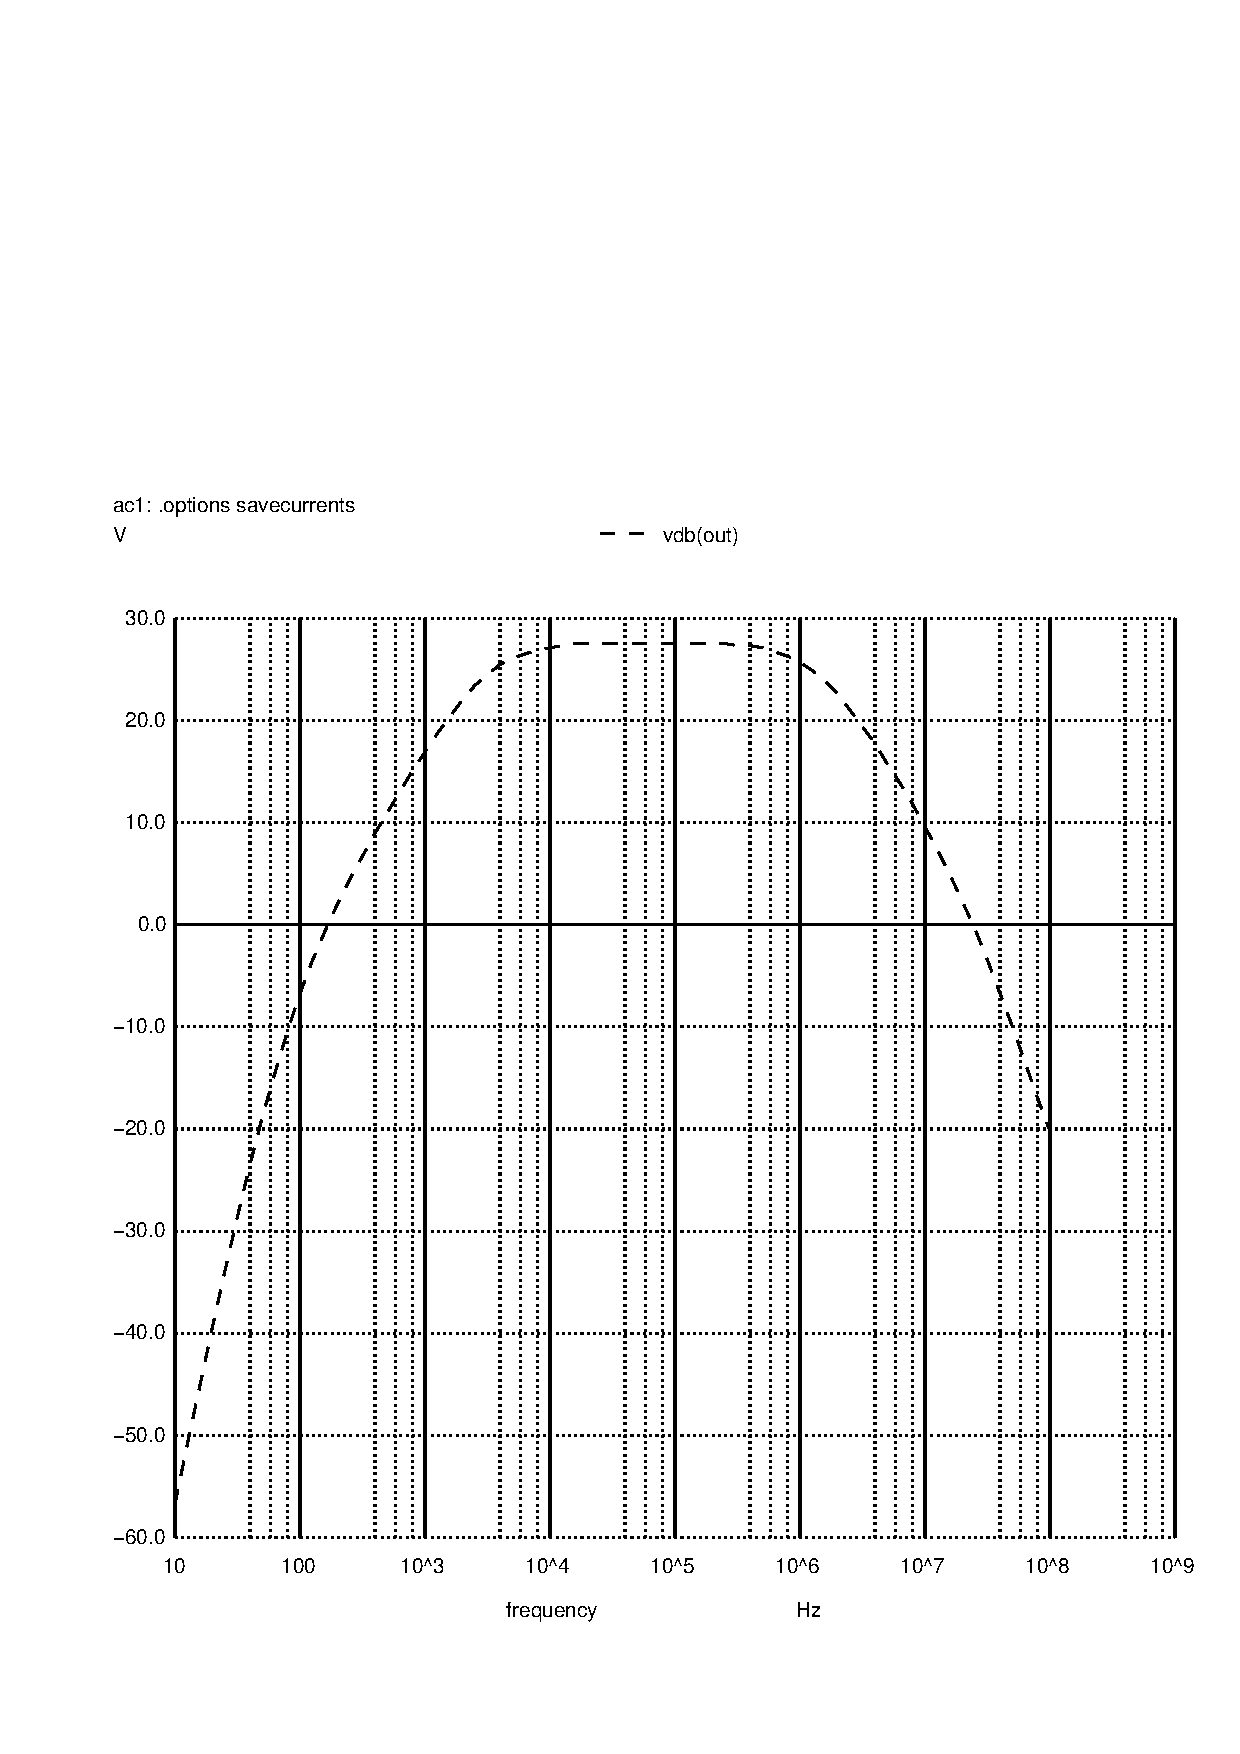
\includegraphics[width = 8cm]{vo2f.pdf} 
\caption{Output}
\label{vo2f}
\end{figure}

\subsection{Merit Results}

From the results obtained through the Ngspice simulation and considering we used the data shown in table 1, we can compute the merit using the formula given in the lab assignment, represented in the Introduction.

The implemented circuit gave us a MERIT of ??? in NGSpice.
The cost equals to ???.

%\begin{table}[H] \centering
%\begin{tabular}{|
%>{\columncolor[HTML]{FFCC67}}l |c|}
%\hline
%\multicolumn{2}{|l|}{\cellcolor[HTML]{EABD8B}Name - Value} \\ \hline
%Cost & 2619.6\\ \hline
merit & 1262.83\\ \hline

%\end{tabular}
%\caption{COST}
%\end{table}



